\documentclass[twoside,11pt,ShortChapTitles]{BYUTextbook}

\usepackage{soul}
\renewcommand{\vec}[1]{\ensuremath{\mathbf{#1}}}
\usepackage{siunitx}
\sisetup{round-mode = figures,
  round-precision = 3, scientific-notation=true}
  \usepackage{marginfix}
  
\usepackage{mathtools}
%\usepackage{amsfonts}
%\usepackage{amsmath}
%\usepackage{graphicx}
%\usepackage{epstopdf}
%\usepackage{amssymb}
%\usepackage{hyperref}
%\usepackage{textcomp}
%\usepackage{listings}
%\usepackage{units}
%\usepackage{color}

%\definecolor{dkgreen}{rgb}{0,0.6,0}
%\definecolor{gray}{rgb}{0.5,0.5,0.5}
%\definecolor{mauve}{rgb}{0.58,0,0.82}

%\lstset{frame=tb,
%  language=Python,
%  aboveskip=3mm,
%  belowskip=3mm,
%  showstringspaces=false,
%  columns=flexible,
%  basicstyle={\small\ttfamily},
%  numbers=none,
%  numberstyle=\tiny\color{gray},
%  keywordstyle=\color{blue},
%  commentstyle=\color{dkgreen},
%  stringstyle=\color{mauve},
%  breaklines=true,
%  breakatwhitespace=true,
%  tabsize=3, upquote=true}

\lstMakeShortInline[columns=fixed]|
\setcounter{chapter}{0}

\begin{document}

\chapter{Measurement and Uncertainty I\label{Measurement and Uncertainty 1}}

\setcounter{page}{1}
\section*{Python You Should Know for This Chapter}
None

\section*{Questions that you should be able to answer by the end of this chapter.}
\begin{enumerate}
\item Given the quantity $8.1\pm0.02\, \text{s}$, what are its {\em value} and {\em error}?

\item What is the difference between being {\em precise} and being {\em accurate}?

\item You measure a cylinder and find that it is $4.2\pm0.05\,\text{cm}$ long and $1.021\pm0.004\,\text{cm}$ in diameter. What is its measured volume (including uncertainty)?  $V_{cyl}=\pi r^2l$

\item You measure the acceleration due to gravity as $10.0 \pm 0.15 \text{m/s}^2$.  What is your percent error?  Was your measurement technique successful?
\end{enumerate}
\hrulefill

\section{The Philosophy of Experimental Measurement}

In experimental measurement, we assume that at a single instant of time that there
is a ``correct" value for some physical
quantity we wish to know. For example, how fast a car is going at a particular
time. The correct value might be something like $64.99999\,\text{mi}/\text{h}$ (because we don't speed here at BYU-I).

The problem is that we can never measure this ``correct" value. That is because no instrument is perfectly
accurate. We have to make do with the goal of getting as close as we can to
the ``correct" value. Your speedometer, for
example, probably would report this speed as $65\,\text{mi}/\text{h}$. But that is not exactly correct.

Several factors\sidenote{Actually there are more factors, but we will deal with the first three in
PH150. PH 250 will deal with computer control and so will likely introduce
quantization error. If you are a physics major, you will take PH336 and deal
with additional error factors.} affect how well we can measure quantities:

\begin{itemize}
\item Proper instruments

\item Instrument calibration

\item Measurement repeatability

\item Quantization error
\end{itemize}



\subsection{Values}

In experimental physics we use the word \emph{value} to mean a number and its
units. For example, we might measure a metal rod and say that the length of
the rod is
\[
L=97.6\,\text{cm}
\]
The number is $97.6$ and the units are centimeters $\left(\text{cm}\right)$. Together they are a value.

Numbers without units are not useful in experimental physics. \textbf{You
should always report both a number and its units.}

\subsection{Errors}

I give you this rod length, all you really know is that the rod is not longer
than about $97.7\,\text{cm} $ or shorter than $97.5\,\text{cm} $ (assuming you trust my ability to measure rods!). Could you be sure that the
rod was not really $97.61\,\text{cm} $ or maybe $97.62\,\text{cm} $?

After making a measurement we have some uncertainty left over because of the
limitation of our instrument. In this case our instrument is a meter stick,
and you know that meter sticks have a smallest tick mark spacing, usually $1\,\text{mm} .$ I could probably judge to within half a millimeter. But it would be kind of
crazy to say that you could be correct to within a $0.000001\,\text{m} $ using a meter stick. Additionally, meter sticks expand and
contract with changes in temperature. So the meter stick itself\sidenote{The meter stick changes in length by about 3 $\mu$m per $^\circ$C} is not
correct to within a hundredth of a millimeter!

One way to express this uncertainty in a measured value is by using
significant figures\sidenote{You have probably done this in high school.  If not, ask one of your classmates or your instructor.}.  As an example:
\[\scalebox{1.5}{$
\overset{\mathclap{\substack{\text{Most Significant Figure} \\ \downarrow}}}{9}7.\underset{\substack{\uparrow \\ \mathclap{\text{Least Significant Figure}}}}{6}\, \text{cm} $}
\]

 We assume the last figure (in this case the $6)$ holds the uncertainty. Think
of making this measurement. You would not be to uncertain about the  $90\,\text{cm}$ represented by the first digit. It is a big mark on the meter stick, and you
could probably tell that the rod was almost a meter long without actually
measuring. You are probably not to uncertain about the  $7\,\text{cm}$ represented by the second digit. You can easily read this from the meter
stick. You will have to count millimeter marks to get the $0.6\,\text{cm} $ represented by the last digit. But it is unlikely that the rod will end
exactly at on the sixth millimeter mark. So this is where our uncertainty
comes in. This is why we call the last digit the least significant digit,
because it is the most uncertain.

If I give you a measurement like $97.6\,\text{cm} $ you would assume that I could be off by $0.1\,\text{cm} $ or by one millimeter. That is what stating $97.6\,\text{cm} $ means. It would be better to state this explicitly\[
L=97.6\pm0.1\,\text{cm}
 \]
But you may object! You can do better than $\pm0.1\,\text{cm} $ with a meter stick. And so can I. This is one reason using significant
figures is not such a great idea. It would be better to state our measurement
and tell the person with whom we are communicating what we think the
uncertainty really is. Say\[
L=97.65\pm0.03\,\text{cm}
 \]
This means that I measured $97\,\text{cm} ,$ then counted up six millimeter marks, and noticed that the rod end landed
at just about half a mark more beyond the sixth mark. I am telling you that I
think because of thermal expansion (and my poor eyesight) that I can only be
sure of this measurement to within about a third of a millimeter.
\textbf{We will always use this notation to report values and their errors in
this class. }If you report a value without an uncertainty, something is wrong
(and the grader will surely notice!). This is because in your actual jobs as
scientists not being clear about how well you know a value can be disastrous,
even causing loss of life or property. So to keep you safe in future jobs, we
will use best practices here.

\subsection{Precision}

So far when we have considered how correct our value is what we have really
been talking about is the \emph{precision} of our measurement. If I measure
the metal rod 50 times, I will get about the same measurement, but not quite,
each time. I might do a poor job of lining up the meter stick and the rod, or
the temperature might change and the meter stick might shrink or expand.
Whatever the problem, each measurement will be a little different. This small
fluctuation about the ``correct" value is
called the precision of the measurement. It tells us how likely it is to get
the same value each time we perform the experiment.

Think of throwing darts. The dots in the next figure represent the location of
five darts from two dart players.

\begin{center}
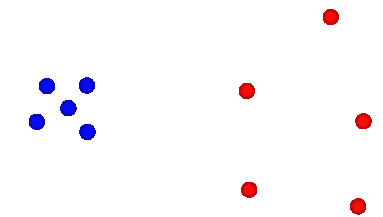
\includegraphics{Lab1_Figs/precVaccur.pdf}
\end{center}

 The blue dots show less spread in their locations than the red dots do. We
would say that the blue dart player was more precise. Another way to say this
is there is less uncertainty in where the blue player's darts will go. In our
notation for reporting a value the plus-or-minus-part is this uncertainty\sidenote{The traditional symbolic notation for an uncertainty in $A$ is either $\delta A$ or $\sigma_A$. Both are used in this manual, and either is ok to use in this course.}:

\[
\scalebox{1.5}{$
A=\overset{\mathclap{\substack{\text{Nominal Value} \\ \downarrow}}}{A}\pm\underset{\mathclap{\substack{\uparrow \\ \text{Uncertainty}}}}{\delta A}
$}
\]

 We call the actual measurement the \emph{nominal value}. That would be where
the dart thrower was aiming. If you know statistics, you can see that this is
a little bit like an average and standard deviation.

Here is another example. Suppose we drive to Idaho falls. The distance is
about 29 miles. If we use our odometer we might find it is marked in 10ths of
a mile. So if I report a drive of 29 miles, I might have gone 29.1 miles, or
28.9 miles. Let's place these on a number line.
\begin{center}
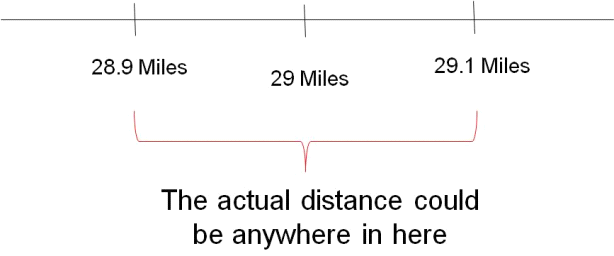
\includegraphics[width=\textwidth]{Lab1_Figs/old_images-003.png}\end{center}
 Notice that my uncertainty is 0.1mile.
\begin{center}
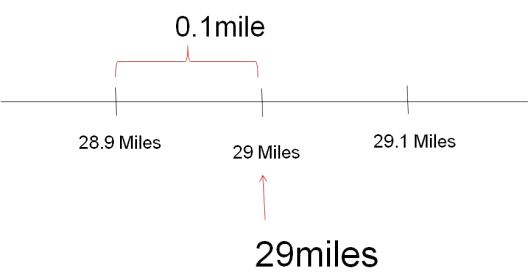
\includegraphics[width=\textwidth]{Lab1_Figs/old_images-004.png}\end{center}
 If the distance is called $d,$ then we write the uncertainty in the distance
by placing the Greek letter $\delta$ in front of our name to get $\delta d.$
This is read ``delta d" or the``uncertainty in $d.$"
\begin{center}
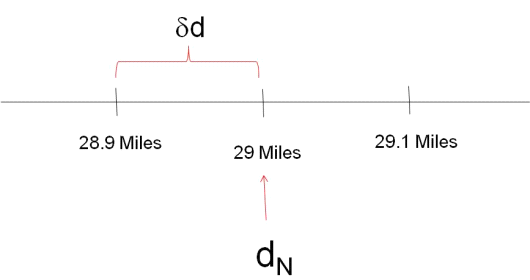
\includegraphics[width=\textwidth]{Lab1_Figs/old_images-005.png}\end{center}
 We name the actual measurement, $d_{N}$ where the $N$ is for ``
nominal value" so then
\[d =d_{N}\pm\delta d=29\pm0.1\,\text{mi} \]


In this case, the $0.1\, \text{mi}$ represents what is called the {\em absolute uncertainty}, and is how we generally report uncertainties.  But, sometimes it is more appropriate to use the {\em relative uncertainty}.  Relative uncertaintity is very useful for judging the quality of your measurement. Here's two examples to illustrate:

First, I measure the distance from Rexburg, ID to Rochester, NY as about
2082.90 miles or $3352100 \text{m}$. Further suppose that I tell you I have made this measurement to $\pm1\,\text{m}$. Is this measurement good?

Now suppose I measure one of our lab tables. I get that the table is  $2\,\text{m}$ long and I tell you that my measurement is good to $\pm1\,\text{m} . $ Is this measurement good?

You can probably see that the first measurement is very good, while the second
measurement could probably have been done better by guessing the length of the
table. It is a terrible measurement with too much uncertainty.

But what makes the difference? The uncertainty is the same in both cases! Of
course the difference is that in one case the uncertainty is a tiny fraction
of the whole value, while in the table case the uncertainty is a large
fraction of the measured value. If the uncertainty is large compared to the
measured value, it is not a good measurement.

But we need a way to communicate this. The error (absolute) is  $\pm1\,\text{m}$
in both cases. Though the
absolute uncertainty can't always tell us the quality of a measurement, we can
use it to calculate
\[
\frac{\delta L}{L}=\text{relative uncertainty}
\]
This gives the error as a percentage of the total measurement. For our Rexburg
to Rochester measurement
\[
\frac{\delta L}{L}=\frac{1\,\text{m} }{352100\,\text{m} }=\allowbreak2.\,\allowbreak840\,1\times10^{-6}
\]
and for the table
\[
\frac{\delta L}{L}=\frac{1\,\text{m} }{2\,\text{m} }=0.5
\]
Since a good measurement has an error that is a small percentage of the total
measurement, we can easily identify which measurement is better by calculating
the percentage of the total value represented by the uncertainty and observing
how small it is. We call this the ``relative
uncertainty." 

The relative uncertainty will be small for a good measurement and large for
a bad one. In this case we can easily see that the Rochester measurement is
much better by looking at the relative uncertainty and noting that it is much
smaller than the table relative uncertainty.

\subsection{Accuracy}

Having a high precision measurement is good, but not enough. Here is a picture
of our darts again, but this time I have included a target. Suppose you were
trying to get a bull's-eye. We can see that our blue dart person is very
precise, but he missed the bull's-eye--and the target! We need more than precision.

\begin{center}
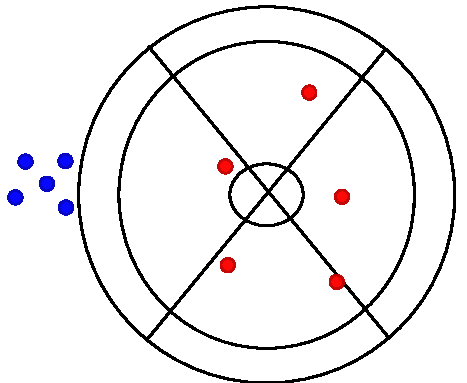
\includegraphics{Lab1_Figs/precVaccur_bulls.pdf}\end{center}

 Notice that if we look at the average location of the red dart dots, the red
dot thrower does seem to be aiming right at the target. We would say that he
is accurate. Accuracy is whether or not you are aiming at the target. If we
drive $29\pm0.1\,\text{mi} $ as we discussed earlier, but we end up in Ashton instead of Idaho Falls, we
would say that no matter how precise our driving distance is, we did not
achieve our goal of getting to Idaho Falls. We mean that we are not accurate.

This might occur in the lab by having a scale that is not zeroed, or a ruler
that is too short or has extra material on the end. The measured amount given
by an instrument when it should be measuring zero is called the``zero offset." If we know about the
problem, we can just adjust the final number by this amount (or re-zero the
instrument). But often we don't know about such problems and they can be hard
to detect.

This type of error is called a \emph{systematic error} because it affects the
system each time it is used. The device will always be off by this amount
until we fix it. We can improve our uncertainty estimate by taking many
measurements and using the average as our value. But if we aim at the wrong
place, no matter how many darts we throw, the accuracy error won't get better.

Of course what we want is both accuracy and precision in our measurements. 

\section{Combining uncertainty}

Suppose I want you to calculate the area of the cover of your text book. That
is easy you say! it is the width times the height. And you are right
\[
A=w\times h
\]
Suppose we measure the book and find it has a height of $h=28.4\,\text{cm} \pm0.2\,\text{cm} $ and a width of $22.2\,\text{cm} \pm0.02\,\text{cm}$. So the area is
\begin{align*}
A  & =28.4\,\text{cm} \times22.2\,\text{cm} \\
& =630.\,\allowbreak48\,\text{cm} ^{2}\end{align*}
but wait, what do we do with the uncertainties? If the initial measurements of
the lengths are uncertain, then the area made from them must be more
uncertain. We need a way to combine our uncertainties for the area.  There are three generally accepted ways to calculate how much our measurement error affects our results\sidenote{Each of these methods fall under the more general term of {\em error propagation} or {\em propagation of error}.}  They are the algebraic method (which is used only in fields where you aren't expected to know calculus) standard or Gaussian error propagation (the gold standard), and Monte Carlo (used when systems are too complex to do standard error propagation).  This chapter will discuss the standard and algebraic methods.

I've also included the ``High/Low Method'' as an example.  You {\bf should never use it in a professional setting}, but it is very good at illustrating how errors in measurement affect your results. 

\subsection{The High/Low Method}

Knowing what our uncertainty means now\sidenote{Reminder: it represents the distance to the poorest
measurements from a group of measurements.}, we can estimate the uncertainty in the area calculated above.  We can guess that if we were off by a positive
$+0.2\,\text{cm} $ on both measurements, then we would have the biggest area we could possibly
get from our measurements. In some way it would be the most off we could get.
Let's call this $A_{\max}.$ We would find it to be
\begin{align*}
A_{\max} &=\left(  28.4\,\text{cm} +0.02\,\text{cm} \right)  \times\left(  22.2\,\text{cm} +0.02\,\text{cm} \right)\\ 
&=28.6\,\text{cm} \times22.4\,\text{cm}\\
&=\allowbreak640.\,\allowbreak64\,\text{cm} ^{2}
\end{align*}


Likewise, if we were off by $-0.2\,\text{cm} $ on both measurements, then we would have the smallest area we could possibly
get from our measurements. In another way it would be the most off we could
get. Let's call this $A_{\min}.$ It would be
\begin{align*}
A_{\min}  & =\left(  28.4\,\text{cm} -0.02\,\text{cm} \right)  \times\left(  22.2\,\text{cm} -0.02\,\text{cm} \right) \\
& =28.2\,\text{cm} \times22.0\,\text{cm} \\
& =\allowbreak\allowbreak620.\,\allowbreak4\,\text{cm} ^{2}\end{align*}
To find the uncertainty, consider our trip to Idaho Falls. We found that the
uncertainty was half the distance between our maximum estimate of our distance
and the minimum estimate of our distance. We can use the same procedure for
our area. We have the maximum and the minimum areas. The uncertainty is half
the difference between these two extremes.\[
\delta A=\frac{A_{\max}-A_{\min}}{2}
\]
using our numbers\begin{align*}
\delta A  & =\frac{\allowbreak640.\,\allowbreak64\,\text{cm} ^{2}-\allowbreak\allowbreak620.\,\allowbreak4\,\text{cm} ^{2}}{2}=10.\,\allowbreak12\,\text{cm} ^{2}\end{align*}
so our area should be reported as
\[
A=630\,\text{cm} ^{2}\pm10\,\text{cm} ^{2}
\]


There are some tricks to this. We have to make sure we have the biggest value
we can get when we get the maximum and the smallest value when we get the
minimum. Suppose I measure two distances $x=1.5\,\text{m} \pm0.3\,\text{m} $ and $y=3.0\,\text{m} \pm0.2\,\text{m} $ and I want to calculate\[
z=\frac{y}{x}
\]
then\begin{align*}
z  & =\frac{3.0\,\text{m} }{1.5\,\text{m} }\\
& =2.0
\end{align*}
what would the uncertainty in $z$ be? Last time we chose adding the plus
uncertainty to both values to get the maximum and we subtracted off both
uncertainty values to get the minimum, but this time lets try every
combination of plus and minus uncertainties
\begin{align*}
\frac{3.0\,\text{m} +0.2\,\text{m} }{1.5\,\text{m} +0.3\,\text{m} }  & =\allowbreak1.\,\allowbreak777\,8\\
\frac{3.0\,\text{m} +0.2\,\text{m} }{1.5\,\text{m} -0.3\,\text{m} }  & =\allowbreak2.\,\allowbreak666\,7\\
\frac{3.0\,\text{m} -0.2\,\text{m} }{1.5\,\text{m} +0.3\,\text{m} }  & =1.\,\allowbreak555\,6\\
\frac{3.0\,\text{m} -0.2\,\text{m} }{1.5\,\text{m} -0.3\,\text{m} }  & =\allowbreak2.\,\allowbreak333\,3
\end{align*}


Note that using both $+$ signs did not give the largest value. That is because
for division a smaller denominator makes the fraction bigger. For the maximum
we want a $+$ in the numerator and a $-$ in the denominator. For the minimum
we want a $-$ in the numerator and a $+$ in the denominator. It is a little
tricky, but if we think, we can find the very biggest possible value and the
very smallest possible value every time. To finish this off, lets find the
uncertainty in $z$

\begin{align*}
\delta z  & =\frac{z_{\max}-z_{\min}}{2}\\
& =\frac{\allowbreak2.\,\allowbreak666\,7-1.\,\allowbreak555\,6}{2}\\
& =\allowbreak0.555\,55
\end{align*}

Now imagine checking every single possible combination of $+$ and $-$ on a more complex equation until you found the highest and lowest values.  The more formal methods avoid that added complexity, and take some statistics\sidenote{They take advantage of the central limit theorem to reduce cross talk between uncertainties, and the fact that it is very unlikely that all of your measurements are at their maximum or minimum value. Any more details on how are beyond the scope of this book.} into account to give a more accurate and consistent way to calculate error.

If you already know how to take a derivative, skip the algebraic method and read the section on Standard Error Propagation.  If you do not yet know how to take a derivative, skip the Standard Error Propagation section and come back to it when you do know how to take a derivative.

\subsection{Algebraic method}
Reminder: if you already know how to take a derivative, jump ahead to the Standard Error Propagation section.


Using algebra, we can develop rules for combining uncertainty when multiplying, dividing, adding, subtracting, or raising variables to whole number powers\sidenote{This is really just multiplying the same value by itself multiple times, so it essentially follows the same rules as multiplication}. These rules will cover many simple situations, but eventually we will need to know how to estimate
uncertainty for any function as explained in the Standard Error Propagation section. But for now our goal is to have a
method that you can use without calculus.

Here are the rules:

\vspace{1 ex}

\begin{tabular}{ccc}
Function &  & Uncertainty Formula\\ \hline
Addition & $z=x+y$ & $\delta z=\delta x+\delta y$\\ \hline
Subtraction & $z=x-y$ & $\delta z=\delta x+\delta y$\\ \hline
Multiplication & $z=xy$ & $\frac{\delta z}{\left\vert z_{N}\right\vert
}=\left(  \frac{\delta x}{x_{N}}+\frac{\delta y}{y_{N}}\right)  $\\ \hline
Division & $z=\frac{x}{y}$ & $\frac{\delta z}{\left\vert z_{N}\right\vert
}=\left(  \frac{\delta x}{x_{N}}+\frac{\delta y}{y_{N}}\right)  $\\ \hline
Multiply by constant & $z=ax$ & $\delta z=a\delta x$\\ \hline
Powers & $z=x^{n}$ & $\frac{\delta z}{\left\vert z_{N}\right\vert }=n\frac{\delta x}{\left\vert x_{N}\right\vert }$\\ \hline
\end{tabular}

\vspace{1 ex}

Here are some examples on how to use the rules.
\subsubsection{Multiplication}
Let's start with the area example from the previous section.  As a reminder, we measured a  book and found that it has a height of $h=28.4\,\text{cm} \pm0.2\,\text{cm} $ and a width of $22.2\,\text{cm} \pm0.02\,\text{cm}$.  To find the area, we use:
\[A = hw= (28.4\,\text{cm})(22.2\,\text{cm}) = 630.48\,\text{cm}^2\]

Applying the multiplication rule to our area formula gives:
\[\frac{\delta A}{A} = \frac{\delta h}{h}+\frac{\delta w}{w} \rightarrow \delta A = \left(\frac{\delta h}{h}+\frac{\delta w}{w}\right)A\]

And now with numbers:
\begin{align*}
\delta A &=\left[ \frac{0.2\,\text{cm}}{28.4\,\text{cm}}+\frac{0.02\,\text{cm}}{22.2\,\text{cm}} \right]\left(630.48\,\text{cm}^2\right)\\
&=\left[0.00704+0.000901\right]\left(630.48\,\text{cm}^2\right) \\
&=5\, \text{cm}^2
\end{align*}

Therefore, the proper way to report the area of the book would be\sidenote{Notice how the value was rounded to match the presicion of the error.}
\[ A = 630 \pm 5\,\text{cm}^2\]

\subsubsection{Addition}
What if instead of finding the area of the book, we wanted to find its perimeter?  For that the formula is:
\[ P = 2h+2w =2\left(28.4\,\text{cm}\right)+2\left(22.2\,\text{cm}\right)=101.2\,\text{cm}\]
Using the addition rule, the formula to find the error would then be\sidenote{Notice that this formula uses both the addition rule {\em and} the multiply by a constant rule.}:
\[\delta P = 2\delta h + 2\delta w = 0.4 \,\text{cm}+0.04\,\text{cm}=0.44\,\text{cm}\]
Therefore, the proper way to report the book's perimeter is:
\[P = 101.2\pm 0.44 \,\text{cm}\]

\subsection{Standard Error Propagation}
Reminder: this section is for those who already know how to take a derivative.  If you do not know calculus, come back to this section when you do.
\subsubsection{Partial Derivatives}
The standard way to do error propagation involves something called a {\em partial derivative}.  If you already know how to do a regular derivative, partial derivatives are almost the exact same thing.  You just change what you consider a constant.  For example,  when taking the regular derivative of $2x^2$, you do this:
\[\frac{d}{dx}2x^2 = 2\frac{d}{dx}x^2 = 2\left(2x\right) = 4x\]
The derivative doesn't do anything to the constant $2$.  To put that into a symbolic form that you might be a little more used to, if $a$ and $n$ are constants,
\[\frac{d}{dx} ax^n = a\frac{d}{dx}x^n = anx^{n-1}\]
Here is that same statement written as a partial derivative:
\[\frac{\partial}{\partial x} ax^n = a\frac{\partial}{\partial x}x^n = anx^{n-1}
\]
 Notice that a partial derivative uses a $\partial$ symbol in place of a $d$. That change in symbols tells you to treat anything that isn't what you are taking a derivative with respect to (in this case, $x$) should be treated as a constant.  Here's an example.  Assuming we have a function $f=5x^2y^3$, our partial derivatives would be:
 \[\begin{aligned}
 \frac{\partial f}{\partial x} &= \frac{\partial}{\partial x}\left[5x^2y^3\right] & = 5y^3\frac{\partial}{\partial x}x^2 &= 10y^3x \\
  \frac{\partial f}{\partial y} &= \frac{\partial}{\partial y}\left[5x^2y^3\right] & = 5x^2\frac{\partial}{\partial y}y^3 &= 15x^2y^2
 \end{aligned}\]
 
 \subsubsection{Calculating Error}
 Here is the traditional\sidenote{It's traditional because it is a very good way to {\em remember} how to calculate the error, not because it is necessarily the best way to {\em learn}.} way of writing out the formula that will calculate the error in any function $f(x,y,z,.....)$:
 \[
 \left(\delta f(x,y,z,....)\right)^2 = \left(\frac{\partial f}{\partial x}\right)^2(\delta x)^2+ \left(\frac{\partial f}{\partial y}\right)^2(\delta y)^2++ \left(\frac{\partial f}{\partial z}\right)^2(\delta z)^2+...
 \]
 
 For any equation, you create the necessary error equation with these steps (an example will follow):
 \begin{enumerate}
 \item Clearly identify which terms in your calculation have an error or uncertainty.
 \item Take the partial derivative of your equation with respect to one of your error terms.
 \item Square the number that you get when you plug your measured values into the partial derivative that you just took..
 \item Multiply the number that you just got by the error in the term you took the derivative with respect to, squared.  (This is one error term)
 \item Repeat for all the measurements for which you have an uncertainty, then add all of the error terms squared
 \item Take the square root of the total
 \end{enumerate}
 
 Here's standard error propagation applied to the book area example from before. As a reminder, we measured a  book and found that it has a height of $h=28.4\pm0.2\,\text{cm} $ and a width of $22.2 \pm0.02\,\text{cm}$.  To find the area, we use:
\[A = hw= (28.4\,\text{cm})(22.2\,\text{cm}) = 630.48\,\text{cm}^2\]

Since both $h$ and $w$ have uncertaintity, we have to take the partial derivative with respect to each of them:
\[\begin{aligned}
\frac{\partial A}{\partial h} &= \frac{\partial}{\partial h} hw&= w\frac{\partial}{\partial h} h &= w\\
\frac{\partial A}{\partial w} &= \frac{\partial}{\partial w} hw&= h\frac{\partial}{\partial w} w &= h
\end{aligned}\]

Now we can calculate the total uncertainty:
\begin{align*}
\left(\delta A\right)^2&=\left(\frac{\partial A}{\partial h}\right)^2\left(\delta h\right)^2+\left(\frac{\partial A}{\partial w}\right)^2\left(\delta w\right)^2\\
&=\left(w\right)^2\left(\delta h\right)^2+\left(h\right)^2\left(\delta w\right)^2\\
&=\left(22.2\,\text{cm}\right)^2\left(0.2\,\text{cm}\right)^2+\left(28.4\,\text{cm}\right)^2\left(0.02\,\text{cm}\right)^2\\
&=19.71\,\text{cm}^4+0.32\,\text{cm}^4\\
&=20.03\,\text{cm}^4\\
\delta A &=\sqrt{20.03}\,\text{cm}^2\\
&=4.5 \,\text{cm}^2
\end{align*}

Therefore, the proper way to quote our calculated area is
\[ A = 630.5 \pm 4.5\,\text{cm}\]
 
\section{Judging success of an experiment}

Now we know how to describe the uncertainty in a measurement and we can even
judge if a measurement is a good one using relative uncertainties. We can find
final uncertainties after a calculation. But how do we know, based on our
measurements, if our experiment is a success?

If we have a known value, we can compare our experimental results to that
known value and judge our accuracy. We do this with a percent error\sidenote{Reminder: You can only use percent error to judge the success of an experiment if you have a known value for comparison.}.
\[
PE=\left(  \frac{\left\|\text{measured value - accepted value}\right\|}{\text{accepted
value}}\times100\right)  \]




We can compare this to our relative uncertainty\[
RE=\left(  \frac{\delta(value)}{\text{nominal value}}\times100\right)  \]
Let's take our drive to IF as an example. Suppose we have a reliable study
that shows the distance to IF is $29.05\,\text{mi} $

\begin{center}
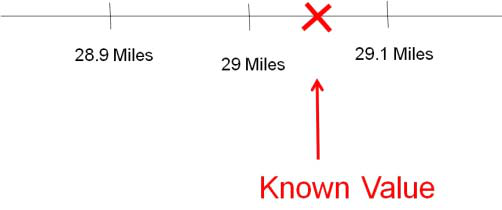
\includegraphics[width=\textwidth]{Lab1_Figs/old_images-008.png}\end{center}
 \bigskip And we go to IF and find that our odometer measures $29\pm0.1\,\text{mi} .$

The percent error is
\begin{align*}
PE  & =\left(  \frac{29.05\,\text{mi} -29\,\text{mi} }{29\,\text{mi} }\times100\right)  \%\\
& =0.172\,41\
\end{align*}
This is roughly a $0.2\%$ error.

Our relative uncertainty is

\begin{align*}
RE  & =\left(  \frac{0.1\,\text{mi} }{29\,\text{mi} }\times100\right)  \%\\
& =\allowbreak0.344\,83\%
\end{align*}

Let's see what this means
\begin{center}
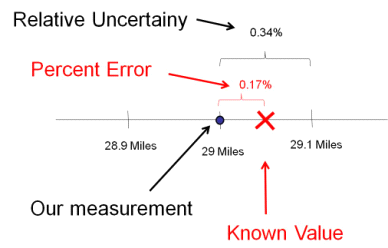
\includegraphics[width=0.8\textwidth]{Lab1_Figs/old_images-009.png}\end{center}
 We can see that we are off from the known value by $0.17\%$, but remember we
are uncertain in our measurement. Our uncertainty tells us we can be anywhere
within $0.34\%$ of the value we measured. Since our percent error--how much we
are off--is less than the fractional uncertainty---percent off we can be based
on our equipment and our technique--we can say that this is an accurate value
for the distance to Idaho Falls. More succinctly: if our percent error is
smaller than our fractional uncertainty, we are accurate.

But suppose our percent error is larger than the relative uncertainty? Then we
are not accurate. It is always good when this happens to try to figure out
what the problem could be. There may be a systematic error, or it may be that
you failed to recognize some source of error.

Here is a rule of thumb for judging the accuracy of an experiment.

\begin{enumerate}
\item If the relative uncertainly is larger than the percent error:

\begin{itemize}
\item The experiment is accurate to within the uncertainty of the experimental technique

\item To improve this measurement, you need better equipment or better technique
\end{itemize}

\item The relative uncertainty is smaller than the percent error:

\begin{itemize}
\item The experiment is not accurate to within the uncertainty of the
experimental technique

\item To improve this experiment, look for systematic errors

\item Consider if you have underestimated the uncertainty
\end{itemize}
\end{enumerate}

We report this along with our results.

In our first lab, we will get some practice calculating uncertainties and
judging accuracies.









\end{document}

% END OF DOCUMENT =======================================================


%SECTION ON LAB NOTEBOOKS =================================================

\section{Lab Notebooks}

Hopefully you noticed that a lab notebook is required for this class. The lab
notebook is designed to be a record of what you did. If you had to repeat
today's experiment five years from now, could you do it based on what you
write today?

At most professional labs and major engineering companies your lab notebook is
considered the property of the company or organization. It is the proof that
you did the experiment that you say you did, and that you got the results you
say you got. It has to be readable and understandable to someone who did not
participate in the lab with you. This is a pretty tall order. To help you plan
your entries, here are the criteria I will use to grade your lab book:

\begin{itemize}
\item Describing the goal for the work

\begin{itemize}
\item Usually this takes the form of a physical law we will test.
\end{itemize}

\item Give predictive equations and uncertainties for the predictions based on
the physical law.

\begin{itemize}
\item This usually involves forming a mathematical model. You should record
any assumptions that went into the model (e.g. no air resistance, point
sources, massless ropes, etc.).

\begin{itemize}
\item In lab today we will find the volume of the room. Your mathematical
model will likely be $V=\ell\times w\times h.$ The mathematical model is not
necessarily something complicated, but the reader needs to know how you are
doing your calculations.
\end{itemize}
\end{itemize}

\item Give your procedure

\begin{itemize}
\item Recording what you really did (not the lab instructions), tell what
changes you make in your procedure as you make them.

\item Record as you do the work.

\item Record the equipment used and settings, values, etc. for that equipment
(see next item).

\item Did you learn how to use any new equipment? What did you learn that you
want to recall later (say, when taking the final, or when you are a
professional and need to use a similar piece of equipment five years from now).
\end{itemize}

\item Record the data you used. The data are all the measurements you took
plus your best estimate of the uncertainties in the measurements. Record any
values you got from tables or published sources (or from your professor) and
state where you got these values. You don't always want to write down all the
data you use. If you have a large set of values, you can place them in a file,
and then record the file name and location in your lab notebook. Make sure
this is a file location that does not change (emailing the data to yourself is
not a good plan).

\item Give a record of the analysis you performed. You should have given some
idea of how you got your predictive equation. Now, what did you do to get the
data through the equation? Were there any extra calculations? Did you obtain a
set of  ``truth data" (data from tables or
published sources, or from an alternate experiment) for your experiment? If
so, did you do any calculations, have any uncertainty, etc. associated with
the truth values?

\item Give a brief statement of your results and their associated uncertainties.

\item Draw conclusions

\begin{itemize}
\item Do your results support the theory? Why or why not? What else did you
learn along the way that you want to record.

\item This is where we may compare the percent error to our relative uncertainty.
\end{itemize}
\end{itemize}


%END SECTION ON LAB NOTEBOOKS ==============================================



%EXCISED MATERIAL==================================================

We can see that if you have $z=x+y$ then you just add the uncertainties
$\delta z=\delta x+\delta y.$ Of course $z$, $x,$ and $y$ stand for any
variable. But how do we know this is true? Here are the details of how the
algebraic method works

\subsubsection{Multiplication}

To multiply two measurements, say\[
m_{measured}=m_{N}\pm\delta m
\]\[
v_{measured}=v_{N}\pm\delta v
\]


We could write these as\[
m_{measured}=m_{N}\left(  1\pm\frac{\delta m}{\left\vert m_{N}\right\vert
}\right)
\]\[
v_{measured}=v_{N}\left(  1\pm\frac{\delta v}{\left\vert v_{N}\right\vert
}\right)
\]


This gives us the measurement in terms of the fractional uncertainties. If we
wish to compute
\[
p=mv
\]
we use
\[
p_{N}=m_{N}v_{N}
\]
but what is the uncertainty in $p?$

The largest value of $p$ is given by\[
p_{\text{large}}=m_{\mathbf{N}}v_{\mathbf{N}}\left(  1+\frac{\delta
m}{\left\vert m_{N}\right\vert }\right)  \left(  1+\frac{\delta v}{\left\vert
v_{\mathbf{N}}\right\vert }\right)
\]
which can be written as\[
p_{\text{large}}=m_{\mathbf{N}}v_{\mathbf{N}}\left(  1+\frac{\delta
m}{\left\vert m_{\mathbf{N}}\right\vert }+\frac{\delta v}{\left\vert
v_{\mathbf{N}}\right\vert }+\frac{\delta v}{\left\vert v_{\mathbf{N}}\right\vert }\frac{\delta m}{\left\vert m_{\mathbf{N}}\right\vert }\right)
\]
We reason that fractional uncertainties should be small, so products of
fractional uncertainties should be very small. We will ignore the very small
term\[
\frac{\delta m}{\left\vert v_{\mathbf{N}}\right\vert }\frac{\delta
m}{\left\vert m_{\mathbf{N}}\right\vert }
\]
so we have\[
p_{\text{large}}=m_{\mathbf{N}}v_{\mathbf{N}}\left(  1+\frac{\delta
m}{\left\vert m_{\mathbf{N}}\right\vert }+\frac{\delta v}{\left\vert
v_{\mathbf{N}}\right\vert }\right)
\]
The smallest value of $p$ is likewise\[
p_{\text{small}}=m_{\mathbf{N}}v_{\mathbf{N}}\left(  1-\frac{\delta
m}{\left\vert m_{\mathbf{N}}\right\vert }-\frac{\delta v}{\left\vert
v_{\mathbf{N}}\right\vert }\right)
\]
In each case we have $m_{\mathbf{N}}v_{\mathbf{N}}$ and then either plus or
minus the term $\frac{\delta m}{\left\vert m_{\mathbf{N}}\right\vert }+\frac{\delta v}{\left\vert v_{\mathbf{N}}\right\vert }$so we have, for our
calculated value of $p$\[
p_{\text{calculated}}=m_{\mathbf{N}}v_{\mathbf{N}}\left(  1\pm\left(
\frac{\delta m}{\left\vert m_{\mathbf{N}}\right\vert }+\frac{\delta
v}{\left\vert v_{\mathbf{N}}\right\vert }\right)  \right)
\]
which we must be able to write as a nominal value and an uncertainty in $p$\[
p_{\text{calculated}}=p_{\mathbf{N}}\left(  1\pm\frac{\delta p}{\left\vert
p_{\mathbf{N}}\right\vert }\right)
\]
Comparing the previous two equations we can see that we must have\[
\frac{\delta p}{\left\vert p_{\mathbf{N}}\right\vert }=\left(  \frac{\delta
m}{m_{\mathbf{N}}}+\frac{\delta v}{v_{\mathbf{N}}}\right)
\]


Then when we multiple measured quantities, we add fractional uncertainties.
This is our algebraic rule for multiplication.

Don't forget, that we need to report $\delta p,$ so to find $\delta p$ we
take\[
\delta p=\frac{\delta p}{\left\vert p_{\mathbf{N}}\right\vert }p_{\mathbf{N}}
\]


\subsubsection{Division}

Let's start again with two measured values $x$ and $y$ with the form\[
x=x_{\mathbf{N}}\left(  1\pm\frac{\delta x}{\left\vert x_{\mathbf{N}}\right\vert }\right)
\]\[
y=y_{\mathbf{N}}\left(  1\pm\frac{\delta y}{\left\vert y_{\mathbf{N}}\right\vert }\right)
\]
We can find the quotient
\[
q=q_{\mathbf{N}}\pm\delta q
\]
as we did for multiplication\[
q=\frac{x_{\mathbf{N}}\left(  1\pm\frac{\delta x}{\left\vert x_{\mathbf{N}}\right\vert }\right)  }{y_{\mathbf{N}}\left(  1\pm\frac{\delta y}{\left\vert
y_{\mathbf{N}}\right\vert }\right)  }
\]
Again find the maximum quotient\[
q_{\text{large}}=\frac{x_{\mathbf{N}}\left(  1+\frac{\delta x}{\left\vert
x_{\mathbf{N}}\right\vert }\right)  }{y_{\mathbf{N}}\left(  1-\frac{\delta
y}{\left\vert y_{\mathbf{N}}\right\vert }\right)  }
\]
and we will play a mathematical trick, we will multiple both top and bottom by
$\left(  1+\frac{\delta y}{\left\vert y_{\mathbf{N}}\right\vert }\right)
,$ since
\[
\frac{\left(  1+\frac{\delta y}{\left\vert y_{\mathbf{N}}\right\vert }\right)
}{\left(  1+\frac{\delta y}{\left\vert y_{\mathbf{N}}\right\vert }\right)
}=1
\]
this will not change our value for $q_{\text{large}}$\[
q_{\text{large}}=\frac{x_{\mathbf{N}}\left(  1+\frac{\delta x}{\left\vert
x_{\mathbf{N}}\right\vert }\right)  }{y_{\mathbf{N}}\left(  1-\frac{\delta
y}{\left\vert y_{\mathbf{N}}\right\vert }\right)  }\frac{\left(
1+\frac{\delta y}{\left\vert y_{\mathbf{N}}\right\vert }\right)  }{\left(
1+\frac{\delta y}{\left\vert y_{\mathbf{N}}\right\vert }\right)  }
\]
The denominator is\[
y_{\mathbf{N}}\left(  1-\frac{\delta y}{\left\vert y_{\mathbf{N}}\right\vert
}\right)  \left(  1+\frac{\delta y}{\left\vert y_{\mathbf{N}}\right\vert
}\right)
\]
We can perform the multiplication to get\begin{align*}
& y_{\mathbf{N}}\left(  1-\frac{\delta y}{\left\vert y_{\mathbf{N}}\right\vert
}+\frac{\delta y}{\left\vert y_{\mathbf{N}}\right\vert }-\frac{\delta
y}{\left\vert y_{\mathbf{N}}\right\vert }\frac{\delta y}{\left\vert
y_{\mathbf{N}}\right\vert }\right) \\
& =y_{\mathbf{N}}\left(  1-\frac{\delta y}{\left\vert y_{\mathbf{N}}\right\vert }\frac{\delta y}{\left\vert y_{\mathbf{N}}\right\vert }\right)
\end{align*}
and we can perform the multiplication in the numerator
\[
x_{\mathbf{N}}\left(  1+\frac{\delta x}{\left\vert x_{\mathbf{N}}\right\vert
}+\frac{\delta y}{\left\vert y_{\mathbf{N}}\right\vert }+\frac{\delta
x}{\left\vert x_{\mathbf{N}}\right\vert }\frac{\delta y}{\left\vert
y_{\mathbf{N}}\right\vert }\right)
\]
so\[
q_{\text{large}}=\frac{x_{\mathbf{N}}\left(  1+\frac{\delta x}{\left\vert
x_{\mathbf{N}}\right\vert }+\frac{\delta y}{\left\vert y_{\mathbf{N}}\right\vert }+\frac{\delta x}{\left\vert x_{\mathbf{N}}\right\vert }\frac{\delta y}{\left\vert y_{\mathbf{N}}\right\vert }\right)  }{y_{\mathbf{N}}\left(  1-\frac{\delta y}{\left\vert y_{\mathbf{N}}\right\vert
}\frac{\delta y}{\left\vert y_{\mathbf{N}}\right\vert }\right)  }
\]
The term\[
\frac{\delta y}{\left\vert y_{\mathbf{N}}\right\vert }\frac{\delta
y}{\left\vert y_{\mathbf{N}}\right\vert }
\]
is very small compared to $1$ (if $\delta y/\left\vert y_{\mathbf{N}}\right\vert $ is a small number, as we assume, then $\delta y^{2}/\left\vert
y_{\mathbf{N}}\right\vert ^{2}$ will be very tiny) so we will drop it from
our calculations (we are calculating uncertainty, the fifth decimal place in
the uncertainty is very uncertain!). We can do this as well with the term\[
\frac{\delta x}{\left\vert x_{\mathbf{N}}\right\vert }\frac{\delta
y}{\left\vert y_{\mathbf{N}}\right\vert }
\]
like we did with the multiplication case. Then\begin{align*}
q_{\text{large}}  & =\frac{x_{\mathbf{N}}\left(  1+\frac{\delta x}{\left\vert
x_{\mathbf{N}}\right\vert }+\frac{\delta y}{\left\vert y_{\mathbf{N}}\right\vert }\right)  }{y_{\mathbf{N}}\left(  1\right)  }\\
& =\frac{x_{\mathbf{N}}}{y_{\mathbf{N}}}\left(  1+\frac{\delta x}{\left\vert
x_{\mathbf{N}}\right\vert }+\frac{\delta y}{\left\vert y_{\mathbf{N}}\right\vert }\right)
\end{align*}
We could go through this again for $q_{\text{small}}$ and we would find
\begin{align*}
q_{\text{small}}  & =\frac{x_{\mathbf{N}}\left(  1-\left(  \frac{\delta
x}{\left\vert x_{\mathbf{N}}\right\vert }+\frac{\delta y}{\left\vert
y_{\mathbf{N}}\right\vert }\right)  \right)  }{y_{\mathbf{N}}\left(  1\right)
}\\
& =\frac{x_{\mathbf{N}}}{y_{\mathbf{N}}}\left(  1-\left(  \frac{\delta
x}{\left\vert x_{\mathbf{N}}\right\vert }+\frac{\delta y}{\left\vert
y_{\mathbf{N}}\right\vert }\right)  \right)
\end{align*}


We can then write\begin{align*}
q_{\text{calculated}}  & =\frac{x_{\mathbf{N}}}{y_{\mathbf{N}}}\left(
1\pm\left(  \frac{\delta x}{\left\vert x_{\mathbf{N}}\right\vert }+\frac{\delta y}{\left\vert y_{\mathbf{N}}\right\vert }\right)  \right) \\
& =q_{\mathbf{N}}\left(  1\pm\frac{\delta q}{\left\vert q\right\vert }\right)
\end{align*}
where
\[
q_{\mathbf{N}}=\frac{x_{\mathbf{N}}}{y_{\mathbf{N}}}
\]
and\[
\frac{\delta q}{\left\vert q\right\vert }=\frac{\delta x}{\left\vert
x_{\mathbf{N}}\right\vert }+\frac{\delta y}{\left\vert y_{\mathbf{N}}\right\vert }
\]
just like the formula for multiplication! The rule is when we divide measured
quantities, we add fractional uncertainties

\subsubsection{Addition}

Let's take two measurements\[
x_{measured}=x_{\mathbf{N}}\pm\delta x
\]\[
y_{measured}=y_{\mathbf{N}}\pm\delta y
\]
and add them to get the largest value of the sum, $z$\begin{align*}
z_{\text{large}}  & =x_{measured}+y_{measured}\\
& =x_{\mathbf{N}}+y_{\mathbf{N}}+\delta x+\delta y
\end{align*}
We can also find the smallest value for $z$\begin{align*}
z_{\text{small}}  & =x_{measured}+y_{measured}\\
& =x_{\mathbf{N}}+y_{\mathbf{N}}-\left(  \delta x+\delta y\right)
\end{align*}
so if we write this as $z_{\mathbf{N}}\pm\delta z$ we have\[
z_{\mathbf{N}}\pm\delta z=x_{\mathbf{N}}+y_{\mathbf{N}}\pm\left(  \delta
x+\delta y\right)
\]
and we can identify
\begin{align*}
z_{\mathbf{N}}  & =x_{\mathbf{N}}+y_{\mathbf{N}}\\
\delta z  & =\left(  \delta x+\delta y\right)
\end{align*}


The rule is that when we add measurements we add their uncertainties.

\subsubsection{Subtraction}

Let's take two measurements\[
x_{measured}=x_{\mathbf{N}}\pm\delta x
\]\[
y_{measured}=y_{\mathbf{N}}\pm\delta y
\]
and add them to get the largest value of the sum, $z$\begin{align*}
z_{\text{large}}  & =x_{measured}-y_{measured}\\
& =\left(  x_{\mathbf{N}}+\delta x\right)  -\left(  y_{\mathbf{N}}-\delta
y\right)
\end{align*}
We can also find the smallest value for $z$\begin{align*}
z_{\text{small}}  & =x_{measured}-y_{measured}\\
& =\left(  x_{\mathbf{N}}-\delta x\right)  -\left(  y_{\mathbf{N}}+\delta
y\right)
\end{align*}
so if we write this as $z_{\mathbf{N}}\pm\delta z$ we have\[
z_{\mathbf{N}}\pm\delta z=x_{\mathbf{N}}-y_{\mathbf{N}}\pm\left(  \delta
x+\delta y\right)
\]
and we can identify
\begin{align*}
z_{\mathbf{N}}  & =x_{\mathbf{N}}-y_{\mathbf{N}}\\
\delta z  & =\left(  \delta x+\delta y\right)
\end{align*}


The rule is that when we subtract measurements, we add their uncertainties
just as we found for addition.

\subsubsection{Measured quantity times an exact number}

Suppose we want the circumference of a circle. We measure the radius to be\[
r_{measured}=r_{\mathbf{N}}\pm\delta r
\]
and we calculate
\[
C_{calculated}=2\pi r_{measured}
\]
how do we determine the uncertainty?

There is not uncertainty in the $2$ nor in the $\pi.$ So we multiply\begin{align*}
C_{calc}  & =2\pi\left(  r_{\mathbf{N}}\pm\delta r\right) \\
& =2\pi r_{\mathbf{N}}\pm2\pi\delta r
\end{align*}
which gives
\[
C_{\mathbf{N}}\pm\delta C=2\pi r_{\mathbf{N}}\pm2\pi\delta r
\]
and we identify
\[
C_{\mathbf{N}}=2\pi r_{\mathbf{N}}
\]
and
\[
\delta C=2\pi\left\vert \delta r\right\vert
\]


In general, if we have
\[
q=Bx
\]
where $B$ is a constant, then we should expect\[
\delta q=\left\vert B\right\vert \delta x
\]


\paragraph{Powers}

For a power, we really are just multiplying\[
y=x^{2}=x\times x
\]
so, taking the fractional uncertainty rule for multiplication,\begin{align*}
\frac{\delta y}{\left\vert y\right\vert }  & =\frac{\delta x}{\left\vert
x\right\vert }+\frac{\delta x}{\left\vert x\right\vert }\\
& =2\frac{\delta x}{\left\vert x\right\vert }\end{align*}


In general, if
\[
y=x^{n}
\]
then
\[
\frac{\delta y}{\left\vert y\right\vert }=n\frac{\delta x}{\left\vert
x\right\vert }
\]

